\subsection{Boosting the Buzz: Enhancing Your Loop Antenna's Voltage!}

\begin{tcolorbox}[colback=gray!10, colframe=black, title=E9H10] How can the output voltage of a multiple-turn receiving loop antenna be increased?
\begin{enumerate}[label=\Alph*.]
    \item By reducing the permeability of the loop shield
    \item By utilizing high impedance wire for the coupling loop
    \item \textbf{By increasing the number of turns and/or the area enclosed by the loop}
    \item All these choices are correct
\end{enumerate} \end{tcolorbox}

\subsubsection*{Concepts Related to the Question}

To understand how to enhance the output voltage of a multiple-turn receiving loop antenna, we need to explore several key concepts in radio communication and antenna theory.

1. \textbf{Antenna Basics:}: Loop antennas are a type of radio antenna that consist of a loop (or multiple loops) of wire, and they are used to receive electromagnetic waves. The output voltage generated by the antenna is proportional to the rate of change of magnetic flux through the loop.

2. \textbf{Number of Turns:}: Increasing the number of turns in a loop antenna is a crucial factor. Each additional turn of wire contributes to the total magnetic flux linkage, thereby enhancing the voltage induced across the antenna. This happens due to the principle of electromagnetic induction, where the induced voltage \(V\) is proportional to the number of turns \(N\):

   \[
   V \propto N \cdot \frac{d\Phi}{dt}
   \]
   
   where \(\Phi\) is the magnetic flux.

3. \textbf{Area of the Loop:}: The voltage induced is also dependent on the area \(A\) enclosed by the loop. A larger area captures more of the magnetic field, resulting in a higher induced voltage:

   \[
   V \propto A \cdot \frac{dB}{dt}
   \]

   where \(B\) is the magnetic field strength.

4. \textbf{Impedance Matching:}: Utilizing high impedance wire for the coupling loop is commonly misunderstood; while it can improve efficiency in some setups, it does not necessarily enhance the output voltage directly.

5. \textbf{Permeability:}: Reducing the permeability of the loop shield can negatively affect performance by reducing the coupling with external magnetic fields.

\subsubsection*{Conclusion}

Therefore, the correct answer to this question is C: By increasing the number of turns and/or the area enclosed by the loop, as these directly contribute to higher output voltage through enhanced magnetic flux linkage.

\begin{center}
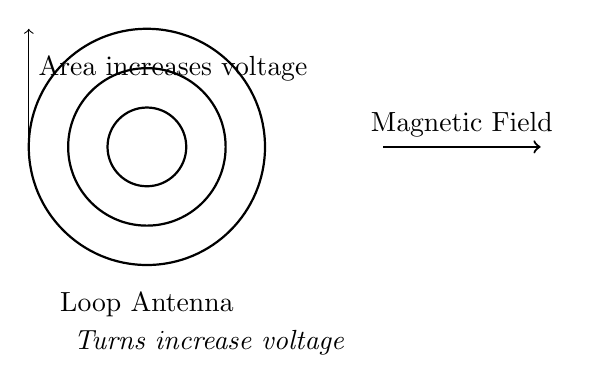
\begin{tikzpicture}
    % Drawing a loop antenna with multiple turns
    \draw[thick] (0,0) circle(1.5);
    \draw[thick] (0,0) circle(1);
    \draw[thick] (0,0) circle(0.5);
    \node at (0,-2) {Loop Antenna};
    \draw[->, thick] (3,0) -- (5,0) node[midway, above] {Magnetic Field};
    \node[below] at (0.8,-2.2) {\textit{Turns increase voltage}};
    \draw[->] (-1.5,0) -- (-1.5,1.5);
    \node[right] at (-1.5,1) {Area increases voltage};
\end{tikzpicture}
\end{center}
